\section{Einführung und Überblick}

\begin{definition}{Software Engineering}
\begin{itemize}
    \item Das Software Engineering (SE) beschäftigt sich mit der Herstellung oder Entwicklung von Software, der Organisation und Modellierung der zugehörigen Datenstrukturen und dem Betrieb von Softwaresystemen
    \item Disziplinen: Anforderungen, Architektur, Implementierung, Test und Wartung
    \item Ziel: Strukturierte Prozesse für Qualität, Risiko- und Fehlerminimierung
    \item Aufgrund des hohen Aufwandes zur Erstellung und Wartung komplexer Software erfolgt die Entwicklung durch Softwareentwickler anhand eines strukturierten (Projekt-)Planes
\end{itemize}
\end{definition}

\begin{KR}{Vorgehen bei der Softwareentwicklung}
\begin{enumerate}
    \item Anforderungen verstehen und dokumentieren
    \item Systemabgrenzung vornehmen
    \item Architektur und Design entwerfen
    \item Implementierung in kleinen, testbaren Schritten
    \item Kontinuierliche Integration und Testing
    \item Regelmäßige Reviews und Refactoring
\end{enumerate}
\end{KR}

\begin{definition}{Modellierung in der Softwareentwicklung}
\begin{itemize}
    \item Modelle als Abstraktionen: Anforderungen, Architekturen, Testfälle
    \item Einsatz von UML für:
    \begin{itemize}
        \item Verstehen eines Gebildes
        \item Kommunizieren über ein Gebilde
        \item Spezifikation von Anforderungen
        \item Durchführung von Experimenten
        \item Aufstellen/Prüfen von Hypothesen
    \end{itemize}
    \item Wieviel Modellierung?: Abhängig von Projektgröße und Komplexität
\end{itemize}
\end{definition}

\begin{example}{Modellierungsaufwand}
Analogie zur Bauplanung:
\begin{itemize}
    \item Hundehütte: Minimale Planung nötig
    \item Einfamilienhaus: Mittlerer Planungsaufwand
    \item Wolkenkratzer: Extensive Planung erforderlich
\end{itemize}
\end{example}

\subsection{Softwareentwicklungsprozesse}

\begin{concept}{Klassifizierung Software-Entwicklungs-Probleme}
Drei Dimensionen beeinflussen die Wahl des Entwicklungsprozesses:
\begin{itemize}
    \item Requirements (Klarheit der Anforderungen)
    \item Technology (Bekanntheitsgrad der Technologie)
    \item People (Erfahrung und Fähigkeiten des Teams)
\end{itemize}
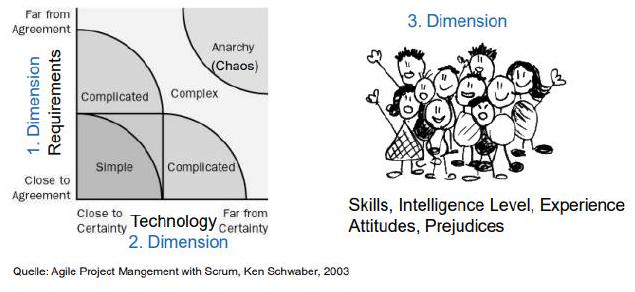
\includegraphics[width=\linewidth]{images/2024_12_29_0d1d7b5551ea1b4b41bdg-01}
\end{concept}

\begin{theorem}{Prozesse im Softwareengineering}
Kernprozesse:
\begin{itemize}
    \item Anforderungserhebung
    \item Systemdesign/technische Konzeption
    \item Implementierung
    \item Softwaretest
    \item Softwareeinführung
    \item Wartung/Pflege
\end{itemize}
\end{theorem}

\begin{corollary}{Unterstützungsprozesse}
\begin{itemize}
    \item Projektmanagement
    \item Qualitätsmanagement
    \item Risikomanagement
\end{itemize}
\end{corollary}

\begin{KR}{Prozessauswahl}
Faktoren für die Wahl des Entwicklungsprozesses:
\begin{enumerate}
    \item Analyse der Projektcharakteristika:
    \begin{itemize}
        \item Projektgröße und Komplexität
        \item Klarheit der Anforderungen
        \item Technologische Risiken
        \item Team-Erfahrung
    \end{itemize}
    \item Wahl des passenden Modells:
    \begin{itemize}
        \item Code \& Fix: Für sehr kleine, experimentelle Projekte
        \item Wasserfall: Für Projekte mit klaren, stabilen Anforderungen
        \item Iterativ-inkrementell: Für komplexe Projekte mit sich entwickelnden Anforderungen
        \item Agil: Für Projekte mit hoher Änderungsdynamik
    \end{itemize}
\end{enumerate}
\end{KR}

[Previous content continues with the definitions of Code and Fix, Wasserfallmodell, etc...]

\begin{concept}{UML in der Praxis}
\begin{itemize}
    \item UML as Sketch: Informelle Diagramme zur Kommunikation
    \item UML as Blueprint: Detaillierte Analyse- und Design-Diagramme
    \item UML as Programming Language: Ausführbare Spezifikationen
\end{itemize}
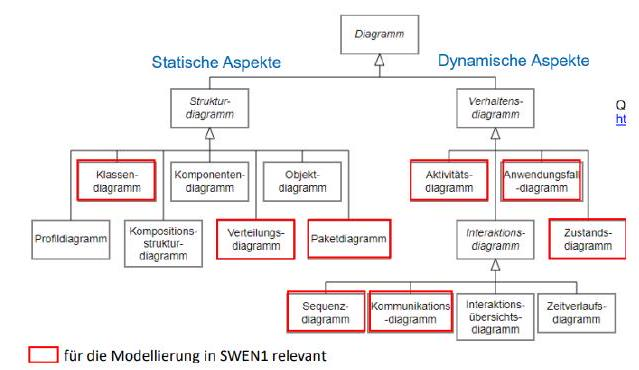
\includegraphics[width=\linewidth]{images/2024_12_29_0d1d7b5551ea1b4b41bdg-01(1)}
\end{concept}

[Previous content continues with the formula for Incremental Model...]

\begin{examplecode}{Typischer Ablauf einer Iteration}
\begin{lstlisting}[language=Java]
// 1. Planungsphase
Iterator<UserStory> stories = iteration.getPlannedStories();
while (stories.hasNext()) {
    UserStory story = stories.next();
    
    // 2. Analyse
    Requirements reqs = story.analyzeRequirements();
    
    // 3. Design
    Design design = story.createDesign();
    
    // 4. Implementierung
    Implementation impl = story.implement(design);
    
    // 5. Testing
    TestSuite tests = story.createTests();
    boolean passed = tests.executeOn(impl);
    
    // 6. Review und Integration
    if (passed) {
        mainBranch.integrate(impl);
    }
}
\end{lstlisting}
\end{examplecode}

\section{Einführung und Überblick}

\begin{definition}{Software Engineering}
\begin{itemize}
    \item Disziplinen: Anforderungen, Architektur, Implementierung, Test und Wartung.
    \item Ziel: Strukturierte Prozesse für Qualität, Risiko- und Fehlerminimierung.
    \item «Zielorientierte Bereitstellung und systematische Verwendung von Prinzipien, Methoden und Werkzeugen für die arbeitsteilige, ingenieurmäßige Entwicklung und Anwendung von umfangreichen Softwaresystemen.» (H. Balzert)
    \item Aufgrund des hohen Aufwandes zur Erstellung und Wartung komplexer Software erfolgt die Entwicklung durch Softwareentwickler anhand eines strukturierten (Projekt-)Planes.
\end{itemize}
\end{definition}

\begin{definition}{Modellierung in der Softwareentwicklung}
\begin{itemize}
    \item Modelle als Abstraktionen: Anforderungen, Architekturen, Testfälle.
    \item Einsatz von UML: Skizzen, detaillierte Blueprints, vollständige Spezifikationen.
    \item Zweck:
    \begin{itemize}
        \item Verstehen eines Gebildes
        \item Kommunizieren über ein Gebilde
        \item Gedankliches Hilfsmittel zum Gestalten, Bewerten oder Kritisieren
        \item Spezifikation von Anforderungen
        \item Durchführung von Experimenten
    \end{itemize}
\end{itemize}
\end{definition}

\begin{KR}{Modellierungsumfang bestimmen}
Folgende Fragen zur Bestimmung des notwendigen Modellierungsumfangs:
\begin{itemize}
    \item Wie komplex ist die Problemstellung?
    \item Wie viele Stakeholder sind involviert?
    \item Wie kritisch ist das System?
    \item Analogie: Planung einer Hundehütte vs. Haus vs. Wolkenkratzer
\end{itemize}
\end{KR}

\begin{example}{Prüfungsfrage zur Modellierung}
Erklären Sie anhand eines selbst gewählten Beispiels, warum der Modellierungsaufwand je nach Projekt stark variieren kann. Nennen Sie mindestens drei Faktoren, die den Modellierungsumfang beeinflussen.

Mögliche Antwort:
\begin{itemize}
    \item Beispiel: Entwicklung einer Smartphone-App vs. Medizinisches Gerät
    \item Faktoren:
    \begin{itemize}
        \item Komplexität der Domäne
        \item Regulatorische Anforderungen
        \item Anzahl beteiligter Stakeholder
        \item Sicherheitsanforderungen
    \end{itemize}
\end{itemize}
\end{example}

[Previous content continues...]

\begin{concept}{Charakteristiken iterativ-inkrementeller Prozesse}
\begin{itemize}
    \item Projekt-Abwicklung in Iterationen (Mini-Projekte)
    \item In jeder Iteration wird ein Stück der Software entwickelt (Inkrement)
    \item Ziele der Iterationen sind Risiko-getrieben
    \item Iterationen werden reviewed und die Learnings fliessen in die nächsten Iterationen ein
    \item Demming-Cycle: Plan, Do, Check, Act
\end{itemize}
\end{concept}

[Rest of previous content...]

\begin{example}{Typische Prüfungsaufgabe: Prozessmodelle vergleichen}
Vergleichen Sie das Wasserfallmodell mit einem iterativ-inkrementellen Ansatz anhand folgender Kriterien:
\begin{itemize}
    \item Umgang mit sich ändernden Anforderungen
    \item Risikomanagement
    \item Planbarkeit
    \item Kundeneinbindung
\end{itemize}

Musterlösung:
\begin{itemize}
    \item Wasserfall:
    \begin{itemize}
        \item Änderungen schwierig zu integrieren
        \item Risiken erst spät erkennbar
        \item Gut planbar durch feste Phasen
        \item Kunde hauptsächlich am Anfang und Ende involviert
    \end{itemize}
    \item Iterativ-inkrementell:
    \begin{itemize}
        \item Flexibel bei Änderungen
        \item Frühes Erkennen von Risiken
        \item Planung pro Iteration
        \item Kontinuierliches Kundenfeedback
    \end{itemize}
\end{itemize}
\end{example}

[Previous formulas and diagrams remain as they were...]